\section{Methods and materials}
\label{sec:methods-and-materials}

% Talk about:
% \begin{itemize}
% \item difference wrt to Barett-Jolley 2011 in terms of channels chosen
% \item availability of code
% \item the fact that we are introducing a ``comprehensive model'' but
%   will only focus on some channels
% \item parameters and their estimation
% \end{itemize}

\subsection{Basic motivation for the model}
\label{sec:model-motivation}

Chondrocytes are the metabolically-active cells found in mature
articular cartilage \citep{BarrettJolleyetal2010}. Articular cartilage
is aneural, avascular, alymphatic connective tissue that covers the
articulating ends of diarthroidal joints \citep{Poole1997,
Mankin1982}. Articular cartilage is thus regularly exposed to
mechanical stresses, and this exposure is essential for the health of
the tissue \citep{Stockwell1991}. Chondrocytes occupy only 1--10\% of
the total volume of articular cartilage in mammals
\citep{CarneyMuir1988, Halletal1996} and play no direct mechanical
role. Mechanical response is provided by the extra-cellular matrix
(ECM) of articular cartilage. The ECM is composed of (a) collagen
fibers, which gives the tissue the ability to resist tension (b)
negatively-charged gel-like proteoglycans (PGs) trapped within the
collagen mesh, allowing the tissue to bear compression
\citep{Poole1997, BuckwaterMankin1998} and (c) synovial fluid within
the articular capsule which acts as a lubricant, allowing for free
movement of the bones \citep{Edwards1994}. The chondrocyte thus
resides in an atypical and dynamic environment and its primary role is
to maintain of viable cartilage tissue by balancing macromolecular
synthesis and breakdown (see e.g. \citet{Wilkinsetal2000,
Stockwell1991, Fassbender1987}). Chondrocytes, like all other cells,
must possess effective membrane transport systems to minimise changes
of cellular composition (in particular, cell volume, pH and ionic
content) in the face of fluctuating surroundings \citep{Halletal1996,
  Mobasherietal1998, Stein1990}. The broad goal of our model is to
explore some of these channels.

\subsection{The atypical environment of the chondrocyte}
\label{sec:chondrocyte-environment}

\begin{itemize}
  \item The high number of fixed negative charges on the proteoglycan
    (GAGs) attract free cations (e.g. Na+) and exclude free anions from
    the matrix. With cation accumulation, water is osmotically imbibed,
    resulting in lowered pH in comparison with other extracellular
    environments \citep{Wilkinsetal2000, LeeUrban1997}.
  \item Extracellular pH affects the chondrocyte metabolism and its
    ability to synthesise the matrix
    \citep{BarrettJolleyetal2010}. However, rate of collagen
    synthesis seems to be independent of pH \citep{Wuetal2007}.
  \item Due to lack of vascularisation, chondrocytes should scavenge
    precursor molecules for matrix macromolecular synthesis
    \citep{Holmetal1998, Stockwell1991}. Synovial fluid supplies adult
    articular cartilage with (small amounts of) nutrients and oxygen
    (and removes byproducts) by diffusion \citep{LeeUrban1997,
      Otte1991}.
  \item Chondrocytes generate ATP by substrate-level phosphorylation
    during anaerobic respiration which generates H+ ions and further
    lowers surrounding pH \citep{LeeUrban1997}.
  \item Mechanical loading during activity exposes chondrocytes to
    profound fluctuations in their physiochemical environment
    \citep{Mowetal1999, Urban1994}.
    Intracellular concentrations too fluctuate with load. The actual
    biophysics of this is relatively uknown. (We will speculate about
    this along with our modelling.)
\end{itemize}

Some experimentally-reported values for the external concentrations of
these different species from are reported in the following tables
\ref{tab:external-concentrations-1} and
\ref{tab:external-concentrations-2}. (We will likely use one of these
tables and values from \cite{Clarketal2011}.)

\begin{table}[ht]
\begin{centering}
\begin{tabular}{r c c c c}
\hline\hline
             & \Nao (mM) & \Ko (mM) & \Cao (mM) & pH\\
\hline
Surface zone & 240--270  & 7--9     & 6--9      & 7.1--7.3\\
Deep zone    & 300--350  & 9--12    & 14--20    & $\sim$6.9\\
\hline
\hline
\end{tabular}
\caption{Experimental ranges of external concentrations
  \citep{Halletal1996}.}
\label{tab:external-concentrations-1}
\end{centering}
\end{table}


\begin{table}[ht]
\begin{centering}
\begin{tabular}{r c c c c}
\hline\hline
             & Cytoplasm & Matrix & Serum/Synovium\\
\hline
\Nao (mM) & 40       & 240--350 & 140\\
\Ko (mM)  & 120--140 & 7--12    & 5\\
\Cao (mM) & 8.e-5 & 6--15 & 1.5\\
$[\mathrm{Cl}^{-}]_{\mathrm{o}} (mM)$ & 60--90 & 60--100 & 140\\
$[\mathrm{HCO^{-}_{3}}]_{\mathrm{o}} (mM)$ & 20 & 15 & 23\\
$[\mathrm{SO^{2-}_{4}}]_{\mathrm{o}} (mM)$ & 0.17 & 0.30 & 0.81\\
pH (mM) & 7.1 & 6.6--6.9 & 7.4\\
Osmolarity (mOsm) & --- & 350--450 & 300\\
\hline
\hline
\end{tabular}
\caption{Experimental ranges of external concentrations
  \citep{Wilkinsetal2000}.}
\label{tab:external-concentrations-2}
\end{centering}
\end{table}

\subsection{Known channels in the chondrocyte}
\label{sec:known-channels}

This will serve as a basis for the features the model can
encompass. (YES: We model this in some fashion. NO: We ignore this for
some valid reason. MAYBE: Not sure what to do about this)

\subsubsection{Potassium channels}

[YES] {\bf Delayed-rectifier $I_{K_{ur}}$}: One of the earliest channels
found in the chondrocyte \citep{Walshetal1992, Sugimotoetal1996,
  Mobasherietal2005a}. These usually repolarize active cells following
action potentials but their role in chondrocytes are not known because
chondrocytes are far more depolarised. Kv 1.4 and 1.6
\citep{Clarketal2010b, Mobasherietal2005a} are known to exist. Others
might as well. \textcolor{red}{Is it ok that we model Kv1.5?}

[YES] {\bf Inwardly-rectifying $I_{K_{ATP}}$}: This channel is closed by
intracellular ATP. It allows for physical coupling between metabolism
and membrane excitability. It is observed to be open in the low-oxygen
tension environment of chondrocytes \citep{DartStanden1994,
  Mobasherietal2007}.

[YES] {\bf Large calcium-activated Potassium $I_{BK}$}: 1. This could
be important for RMP. 2. Could act as an ``osmolyte channel''
$\rightarrow$ K+ ions leave $\rightarrow$ decrease intracellular
osmotic potential $\rightarrow$ regulatory volume decrease. 3. Could
be a stretch-activated channel. Stretch $\rightarrow$ increased
calcium $\rightarrow$ increased BK current. (Many citations and
speculations in \citet{BarrettJolleyetal2010}.)

[NO] {\bf Small calcium-activated Potassium $I_{SK}$}: A few reports
suggest this might exist \citep{Halletal1996,
  BarrettJolleyetal2010}. Tiny magnitude, by definition and role
unknown. So we ignore it.

\subsection{Model Development}
\label{sec:model-development}

In this discourse, we focus our attention on a single chondrocyte cell
residing in deep regions of cartilage. This cartilage environment is
modelled simply by (fixed) external concentrations \Nao, \Ko, \Cao,
and \Ho. Values for these concentrations are chosen within
physiologically-relevant ranges (see
Table~\ref{tab:external-concentrations}). We are interested in
studying the behaviour of cell under this environment, in particular
looking at how the flux of these ions through membrane channels
changes their internal concentrations over time and how this changes
the cell's membrane potential. The channels under consideration are
illustrated in Figure~\ref{fig:chondrocyte-model}.

\begin{figure}[ht]
  \centering
  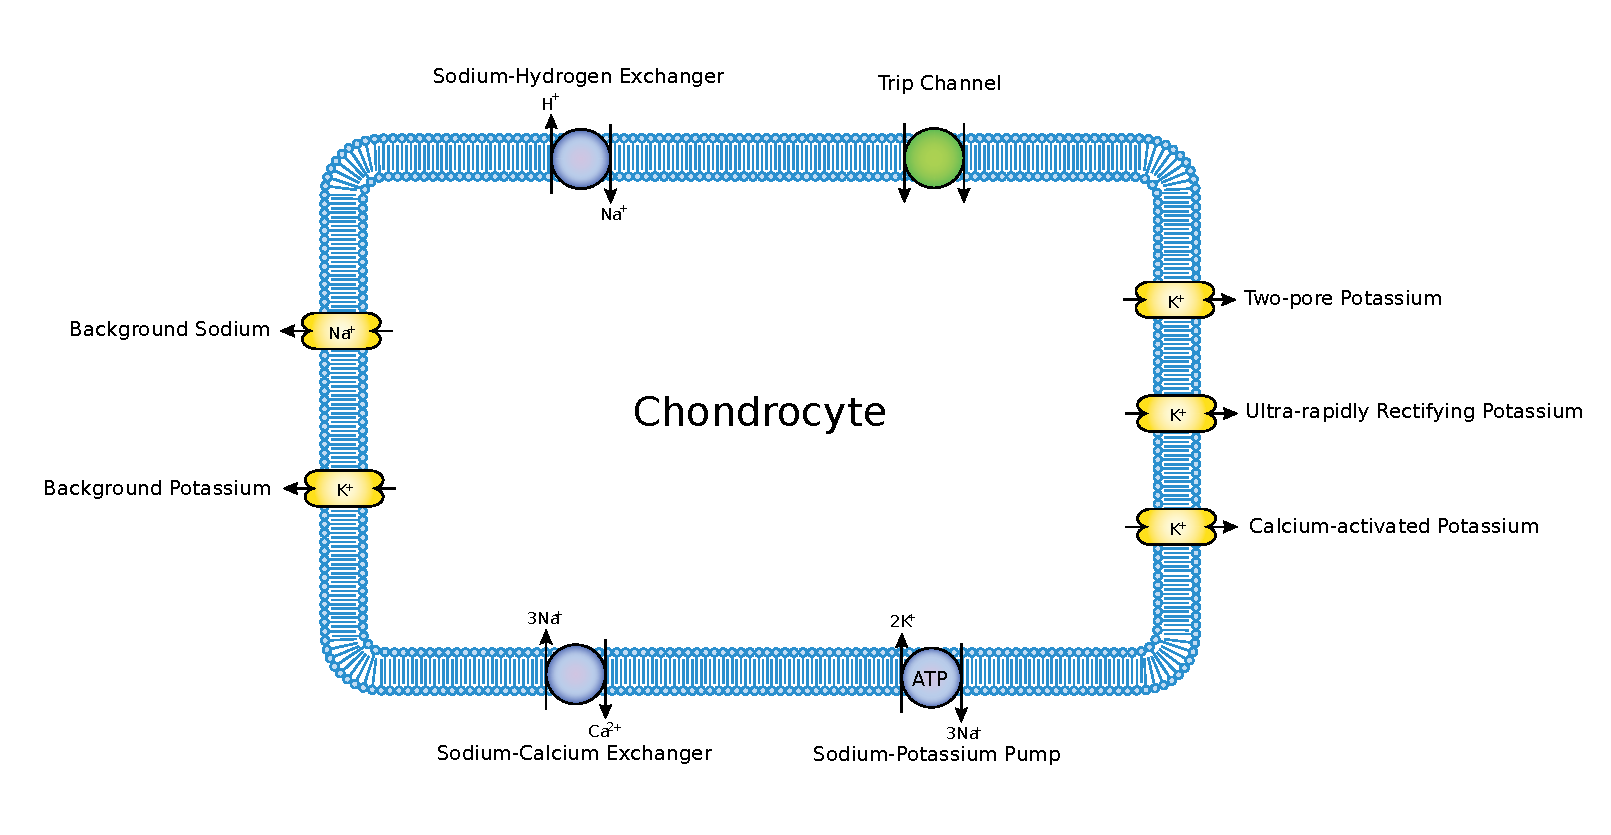
\includegraphics[width=\textwidth]
  {../images/pdf/chondrocyte-model-cellml}
  \caption{An illustration of the model.}
  \label{fig:chondrocyte-model}
\end{figure}

In order to simplify the treatment, we assume that there are no
spatial variations in these quantities of interest, allowing us to
model the cell as the following set of ordinary differential equations
(ODEs) in time.

\begin{equation}
  \frac{d}{dt}
  \left(
    \begin{array}{c}
      V_{\rm m}\\
      \left[Na^{+}\right]_{i}\\
      \left[\rm K^{+}\right]_{i}\\
      \left[\rm Ca^{2+}\right]_{i}\\
      \left[\rm H^{+}\right]_{i}\\
      a_{\rm ur}\\
      i_{\rm ur}\\
    \end{array}
  \right)  = \left(
    \begin{array}{c}
        (-I_{i} + I_{\rm stim})/{C_{\rm m}}\\
      - (I_{\rm Na_{b}} + 3\, I_{\rm NaK} + 3\, I_{\rm NaCa} - I_{\rm
        NaH})/(v_{i}\, F)\\
      - (I_{\rm K_{b}} - 2\, I_{\rm NaK} + I_{\rm K_{ur}} + I_{\rm
        K_{2\, pore}} + I_{\rm K_{Ca-act}} + I_{\rm K_{ATP}})/(v_{i}\,
      F)\\
        (I_{\rm NaCa})/(v_{i}\, F)\\
      - (I_{\rm NaH})/(v_{i}\, F)\\
      (a_{{\rm ur}_{\infty}} - a_{\rm ur})/\tau_{a_{\rm ur}}\\
      (i_{{\rm ur}_{\infty}} - i_{\rm ur})/\tau_{i_{\rm ur}}\\
    \end{array}
  \right)
\end{equation}

\noindent where,

\begin{displaymath}
    \begin{split}
      I_{i} =
      & \phantom{+\,} \underbrace{I_{\rm Na_b} + I_{\rm K_b}}_{\rm
        Background\, currents}\\
      & +\, \underbrace{I_{\rm NaK} + I_{\rm NaCa} + I_{\rm NaH}}_{\rm
        Pumps\, and\, exchangers}\\
      & +\, \underbrace{I_{\rm K_{ur}} + I_{\rm K_{2\, pore}} + I_{\rm
          K_{Ca-act}} + I_{\rm K_{ATP}}}_{\rm Potassium\, channels}\\
      & +\, \underbrace{I_{\rm ASIC} + I_{\rm TRP1} + I_{\rm TRP2} +
        I_{\rm stim}}_{\rm Other\, currents}
    \end{split}
\end{displaymath}

This ODE system is solved for the primary vector of unknowns: $V_{\rm
m}$, $Na_{\rm i}$, $K_{\rm i}$, $Ca_{\rm i}$, $H_{\rm i}$, $a_{\rm
ur}$, $i_{\rm ur}$.

\subsection{Background Currents}
\label{sec:background-currents}

Background Sodium Current (Hodgkin Huxley?):
\begin{equation}
  \begin{split}
    I_{\rm Na_b} & = \bar{g}_{\rm Na_b} (V_{\rm m} - E_{\rm Na})\\
    E_{\rm Na} & =  \frac{R T}{z_{\rm Na} F}
    \ln\left(\frac{\left[Na^{+}\right]_{o}}
      {\left[Na^{+}\right]_{i}}\right)
  \end{split}
\end{equation}

Background Potassium Current (Hodgkin Huxley?):
\begin{equation}
  \begin{split}
    I_{\rm K_b} & = \bar{g}_{\rm K_b} (V_{\rm m} - E_{\rm K})\\
    E_{\rm K} & =  \frac{R T}{z_{\rm K} F}
    \ln\left(\frac{\left[K^{+}\right]_{o}}
      {\left[K^{+}\right]_{i}}\right)
  \end{split}
\end{equation}

\subsection{Pumps and exchangers}
\label{sec:pumps-and-exchangers}

Sodium Potassium Pump \citep[Table 12, pp. 77]{Nygrenetal1998}:
\begin{equation}
  I_{\rm NaK} =
  \bar{I}_{\rm NaK} \left( \frac{[\rm K^{+}]_{\rm o}}{[\rm K^{+}]_{\rm o} +
    k_{\rm NaK_{K}}} \right) \left(\frac{[\rm Na^{+}]^{1.5}_{\rm i}}{[\rm
    Na^{+}]^{1.5}_{\rm i} + k^{1.5}_{\rm NaK_{Na}}}\right) \left( \frac{V + 150}{V +
    200} \right)
\end{equation}

Sodium Calcium Exchanger \citep[Table 13, pp. 77]{Nygrenetal1998}:
\begin{equation}
  I_{\rm NaCa} = k_{\rm NaCa} \frac{[\rm Na^{+}]^{3}_{i}[\rm
    Ca^{2+}]_{o} \exp(\frac{\gamma V F}{R T}) - [\rm
    Na^{+}]^{3}_{o}[\rm Ca^{2+}]_{i} \exp(\frac{(\gamma - 1.0) V F}{R
      T})} {1.0 + d_{\rm NaCa}([\rm Na^{+}]^{3}_{o}[\rm Ca^{2+}]_{i} +
    [\rm Na^{+}]^{3}_{i}[\rm Ca^{2+}]_{o})}
\end{equation}

Sodium Hydrogen Exchanger \citep[Eq. 2, pp. 2675]{Chaetal2009}
\begin{equation}
  \begin{split}
    I_{{\rm NaH}_{\rm mod}} & = \frac{1}{1 + (K_{\rm i}^{n_{\rm
          H}}/[{\rm H}^{+}]_{\rm i}^{n_{\rm H}})}\\
    t_{1} & = \frac{k_{1}^{+} [{\rm Na}^{+}]_{\rm o}/K_{\rm Na}^{\rm
        o}} {(1 + [{\rm Na}^{+}]_{\rm o}/K_{\rm Na}^{\rm o} + [{\rm
        H}^{+}]_{\rm o} /K_{\rm H}^{\rm o})}\\
    t_{2} & = \frac{k_{2}^{+} [{\rm H}^{+}]_{\rm i}/K_{\rm H}^{\rm i}}
    {(1 + [{\rm Na}^{+}]_{\rm i}/K_{\rm Na}^{\rm i} + [{\rm
        H}^{+}]_{\rm i}/K_{\rm H}^{\rm i})}\\
    t_{3} & = \frac{k_{1}^{-} [{\rm Na}^{+}]_{\rm i}/K_{\rm Na}^{\rm
        i}} {(1 + [{\rm Na}^{+}]_{\rm i}/K_{\rm Na}^{\rm i} + [{\rm
        H}^{+}]_{\rm i} /K_{\rm H}^{\rm i})}\\
    t_{4} & = \frac{k_{2}^{-} [{\rm H}^{+}]_{\rm o}/K_{\rm H}^{\rm
        o}} {(1 + [{\rm Na}^{+}]_{\rm o}/K_{\rm Na}^{\rm o} + [{\rm
        H}^{+}]_{\rm o} /K_{\rm H}^{\rm o})}\\
    I_{{\rm NaH}_{\rm exch}} & = \frac{(t_1 t_2 - t_3 t_4)}
    {(t_1 + t_2 + t_3 + t_4)}\\
    I_{\rm NaH} & = N_{\rm NaH} I_{\rm NaH_{\rm mod}}
    I_{\rm NaH_{\rm exch}}
  \end{split}
\end{equation}

\subsection{Potassium channels}
\label{sec:potassium-channels}

Ultra-rapidly rectifying potassium channel \citep{Maleckaretal2009}:
\begin{equation}
  \begin{split}
    I_{\rm K_{\rm ur}} & = g_{\rm K_{\rm ur}}\, a_{\rm ur}\, i_{\rm
      ur}\, (V - E_{\rm K})\\
    E_{\rm K} & =  \frac{R T}{z_{\rm K} F}
    \ln\left(\frac{\left[K^{+}\right]_{o}}
      {\left[K^{+}\right]_{i}}\right)\\
    a_{{\rm ur}_{\infty}} & = \frac{1}{1 + \exp(-(V_{\rm m} +
      6.0)/8.6)}\\
    i_{{\rm ur}_{\infty}} & = \frac{1}{1 + \exp(-(V_{\rm m} +
      7.5)/10.0)) + 0.7}\\
    \tau_{a_{\rm ur}} & = \frac{0.009}{1 + \exp((V + 5.0)/12.0)} +
    0.0005\\
    \tau_{i_{\rm ur}} & = \frac{0.5}{1 + \exp((V +60.0)/20.0)} +
    6\\
  \end{split}
\end{equation}

Two-pore potassium channel \citep{UNKNOWN}:
\begin{equation}
 I_{\rm K_{2\, pore}} = P_{\rm K}\, \frac{z_{\rm K}^2\, V\, F^{2}}{R\,
   T}\, \frac{({\left[K^{+}\right]_{i}} - {\left[K^{+}\right]_{o}}\,
 exp(\frac{-z_{\rm K}\, V\, F}{R\, T}))}{(1 - \exp(-z_K\, V\, F/(R\,
 T))} + I_{{\rm K_{2\, pore}}_0}
\end{equation}

Calcium-activated potassium channel \citep{HorriganAldrich2002}:
\begin{equation}
  \begin{split}
    kTe & = 23.54\, (T/273)\\
    L_v & = L0\, \exp((V\, Z_L)/kTe)\\
    J_v & = \exp(((V - Vh_j)\, Z_j)/kTe)\\
    K & = Ca_i/KDc\\
    P_0 & = \frac{L_v\, (1+K\, C+J_v\, D+J_v\, K\, C\, D\, E)^4}
    {L_v\, (1+K\, C+J_v\, D+J_v\, K\, C\, D\, E)^4 +
      (1+J_v+K+J_v\, K\, E)^4}\\
    E_{\rm K} & =  \frac{R T}{z_{\rm K} F}
    \ln\left(\frac{\left[K^{+}\right]_{o}}
      {\left[K^{+}\right]_{i}}\right)\\
    I_{\rm K_{Ca-act}} & = N_{\rm K_{Ca-act}}\, P_0\, G_{\rm max}\, (V -
    E_{\rm K})
  \end{split}
\end{equation}

Potassium pump \citep{UNKNOWN}:
\begin{equation}
  I_{\rm K_{ATP}} =
\end{equation}

\subsection{Other channels}
\label{sec:other-channels}

Voltage-activated hydrogen channel \citep{UNKNOWN}:
\begin{equation}
  I_{\rm ASIC} =
\end{equation}

Stretch-activated trip channel \citep{UNKNOWN}:
\begin{equation}
  I_{\rm TRP1} = \bar{g}_{\rm TRP1}\, (V_{\rm m} - E_{\rm ?})
\end{equation}

Osteo-arthritic trip channel \citep{UNKNOWN}:
\begin{equation}
  I_{\rm TRP2} = \bar{g}_{\rm TRP2}\, (V_{\rm m} - E_{\rm ?})
\end{equation}

External stimulation (matching experiments, e.g. cyclic stimulation):
\begin{equation}
I_{\rm stim} = \overline{I_{\rm stim}}\, {\rm square}(\frac{2 \pi\,
  t}{t_{\rm cycle}}, \frac{t_{\rm stim}}{t_{\rm cycle}})
\end{equation}

% \begin{sidewaystable}[ht]
% \begin{tabular}{r c l l}
% \hline\hline
% Current description & Notation & Functional form & Parameter values \\ [0.5ex]
% \hline
% Background sodium & $I_{\rm Na_b}$ & $\bar{g}_{\rm Na_b} (V_{\rm m} - E_{\rm Na})$ \cite{UNKNOWN}
%                           & $\bar{g}_{\rm Na_b} = $ \cite{UNKNOWN}, $E_{\rm Na} = $ \cite{UNKNOWN}\\
% Background potassium & $I_{\rm K_b}$ & $\bar{g}_{\rm K_b} (V_{\rm m} - E_{\rm K})$ \cite{UNKNOWN}
%                           & $\bar{g}_{\rm K_b} = $ \cite{UNKNOWN}, $E_{\rm K} = $ \cite{UNKNOWN}\\
% Sodium-potassium pump & $I_{\rm NaK}$ & $\bar{I}_{\rm NaK}
% \frac{[\rm K^{+}]_{\rm c}}{[\rm K^{+}]_{\rm c} + k_{\rm NaK_{K}}}
% \frac{[\rm Na^{+}]^{1.5}_{\rm i}}{[\rm Na^{+}]^{1.5}_{\rm i} + k^{1.5}_{\rm
%     NaK_{Na}}}
% \frac{V + 150}{V + 200}$\cite{Nygrenetal1998} & \cite{Nygrenetal1998}\\
% Sodium-calcium exchanger & $I_{\rm NaCa}$ & $k_{\rm NaCa}
% \frac{[\rm Na^{+}]^{3}_{i}[\rm Ca^{2+}]_{c} \exp(\frac{\gamma V F}{R T}) -
% [\rm Na^{+}]^{3}_{c}[\rm Ca^{2+}]_{i} \exp(\frac{(\gamma - 1.0) V F}{R T})}
% {1.0 + d_{\rm NaCa}([\rm Na^{+}]^{3}_{c}[\rm Ca^{2+}]_{i} + [\rm
%   Na^{+}]^{3}_{i}[\rm Ca^{2+}]_{c})}$
% \cite{Nygrenetal1998} & \cite{Nygrenetal1998}\\
% Sodium-hydrogen exchanger & $I_{\rm NaH}$ & \cite{UNKNOWN} & \cite{UNKNOWN}\\
% Ultra-rapidly rectifying potassium & $I_{\rm K_{ur}}$ & $g_{\rm
%   K_{ur}}\, a_{\rm ur}\, i_{\rm ur}\, (V_{\rm m} - E_{\rm K})$ \cite{Maleckaretal2009} & \cite{Maleckaretal2009}\\
% Two-pore potassium channel & $I_{\rm K_{2\, pore}}$ & \cite{UNKNOWN} & \cite{UNKNOWN}\\
% Calcium-activated potassium & $I_{\rm Ca_{act}K}$ & \cite{UNKNOWN} & \cite{UNKNOWN}\\
% Trip channel(s) & $I_{\rm TRP}$ & $\bar{g}_{\rm NaCa_{TRP}}\, (V_{\rm
%   m} - E_{\rm NaCa})$ \cite{UNKNOWN} & \cite{UNKNOWN}\\
% Applied stimulus & $ I_{\rm stim}$ & Mirroring experiments \cite{Clarketal2011} &  --- \\ [1ex]
% \hline
% \end{tabular}
% \caption{Details of the model}
% \label{tab:chondrocyte-model-details}
% \end{sidewaystable}

% Local Variables:
% TeX-master: "chondrocyte-model"
% mode: latex
% mode: flyspell
% End:
